\documentclass[11pt, letterpaper, twocolumn]{article}

% Input
\usepackage[english]{babel}
\usepackage[utf8]{inputenc}
% Geometry
\usepackage[margin=1.0in]{geometry}
\usepackage{titlesec}
\titleformat*{\section}{\large\bfseries}
\titleformat*{\subsection}{\bfseries}
% Fonts
%\usepackage{fontspec}
%xs\setmainfont{Arial}
% Figures and Symbols
\usepackage{graphicx}
\usepackage{caption}
\captionsetup[figure]{font=small}
\usepackage{amsmath}
\usepackage{amssymb}
\usepackage[]{siunitx}
% Misc
\usepackage{epigraph}
% Fancy Header
\usepackage{fancyhdr}
\setlength{\headheight}{14.5pt}
\pagestyle{fancy}
\fancyhf{}
% \renewcommand{\headrulewidth}{0pt}

\lhead{Fluid Simulation in CG WS2020 - RWTH Aachen } 
\rhead{Group 4: Ertural, Ledwon} 
\rfoot{\thepage}


\begin{document}
% Title, Abstract
\twocolumn[
\begin{@twocolumnfalse}
  \begin{center}
    \textbf{\large{Report: Fluid Simulation in Computer Graphics WS2020}}\\
    \vspace{0.1cm}
    \textbf{\small{Weakly Compressible Smoothed Particle Hydrodynamics
        \\and Position Based Fluids}}\\
    \vspace{0.2cm}
    \small{Berat Ertural, Dennis Ledwon\\
      RWTH Aachen, Visual Computing Institute\\
      Supervisor: Jose Antonio Fernandez Fernandez\\}

    \epigraph{Reading maketh a full man; conference a ready man; and writing an exact man.}
{\textit{Sir Francis Bacon}}
  \end{center}
\end{@twocolumnfalse}
]


\section{Introduction} \label{sec:introduction}

Fluids play a vital role in our lifes. Understanding the motion and behaviour of fluids is not only crucial to many fields of engineering, but it also aids us in creating beautiful virtual worlds, such as used in games and cinema. The simulation of fluids is a vast and rapidly growing field. During the course of this practical, we implemented two different fluid solvers and evaluated their characteristics.

The motion of fluids is governed by the famous Navier-Stokes equation, as given below in its Lagrangian form;
\begin{equation}
  \mathbf{\dot{v}}_i = \frac{\partial v_i}{\partial t} = -\frac{1}{\rho_i}\nabla p_i +\nu \nabla^2 \mathbf{v}_i + \frac{F^{ext}_i}{m_i}.
\end{equation}
The Lagrangian form denotes the sampling points as dynamic particles moving with the flow of the fluid. The above partial differential equation (PDE) describes the acceleration \( \dot{v}_i\) of such a particle \( i \) as depending on the internal pressure gradient \( \nabla p_i\) and the veloctity divergence \( \nabla^2 \mathbf{v}_i\) of the fluid. The velocity divergence and friction coefficient \( \nu \) represent the viscoscity of the fluid due to internal friction. The pressure gradient drives the acceleration due to internal pressure differences, to achieve incompressebility. In theory the density of the fluid is said to be constant, 
\(\frac{\delta \rho}{\delta t} = 0\).
In practice, absolute incompressebility is not achievable due to numerical errors \cite{bender2015}. Sometimes, small deviations of particle densities from the rest density of the fluid are desirable \cite{ihmsen2014}. 

As with many PDE describing natural phenomena, the Navier-Stokes equation has no analytical solution. Nonetheless, numerical approximations to fluid dynamics exist and during the course of the practical lecture we were tasked to implement two such solvers, namely Weakly Compressible Smoothed Particle Hydrodynamics (WCSPH) \cite{ihmsen2014} and Position based Fluids (PBF) \cite{macklin2013}. 
In the next section, we will give a short overview of the used methods and implementation of the application.
We will then show the results of our experiments that were designed to demonstrate the differences between the WCSPH and the PBF solver and the impact of simulation parameters on the fluid behavior in Sec. \ref{sec:results}. In Sec. \ref{sec:discussion}, we provide interpretations for the 
results of these experiments. Finally, we give concluding remarks and an outlook in Sec. \ref{sec:conclusion} and Sec. \ref{sec:future}.



\section{Methods} \label{sec:methods}
In the following, a short overview of the methodological background and implementation will be given. In addition, certain aspects of the implementation that differ from the instructions given on our assignment sheets will be presented.
For a thorough discussion of the SPH and PBF framework we refer the reader to the review of SPH fluids by Ihmsen et al. \cite{ihmsen2014} and to the original paper about PBF by Macklin et al. \cite{macklin2013}, as well as the works of Akinci et al. \cite{akinci2012, akinci2013}.

\subsection{Weakly Compressible SPH}
\label{subsec:wcsph}
Smoothed Particle Hydrodynamics (SPH) is a class of particle based methods for fluid simulation with a long record of scientific publications.
The core idea of SPH is to approximate any attribute \( A_i\) of a point at an arbitrary position \(\mathbf{x}_i\) by weighting the attributes of the immediate surrounding particles \(j \in N \);
\begin{equation}
  A_i = \sum_{j \in N} \frac{m_j}{\rho_j}  A_j \cdot  W(||\mathbf{x}_i - \mathbf{x}_j||/h).
  \label{eq:weight}
\end{equation}
Here, $m_j / p_j$ is used as a normalization factor.
The weighting is performed by the so called kernel function \( W : \mathbb{R} \rightarrow \mathbb{R}\), with \(W(q) = \frac{1}{h^3}f(q)\), 
where $q$ is the ratio of the distance between two particles and the smoothing length \(h\), which is a multiple of the particle diameter; \(h = \mu \cdot 2r\).
We set \(\mu = 1.2\), during the remainder of this report.
The function $f$ that is used in the computation of the kernel weights is the following cubic spline \cite{monaghan1992},
\begin{equation}
  f(q) = \frac{3}{2\pi}
  \begin{cases}
    \frac{2}{3} - q^2 + \frac{1}{2}q^3 & 0 \leq q < 1 \\
    \frac{1}{6}(2-q)^3 & 1 \leq q < 2 \\
    0 & 2 \leq q \\
  \end{cases}
  .
\end{equation}
It should be noted, that the effective radius of the kernel function, and therefore the number of neighbourhood particles taken into account during the computation of a particle attribute, depends on the smoothing length.
Weakly Compressible SPH first computes the particle density \(\rho_i\) using (\ref{eq:weight}) and then applies it to a so called Equation of State (EOS) to derive the resulting particle pressures \(p_i\). In the application the following EOS was used to derive the pressures;
\begin{equation}
  p_i = max(0, B(\rho_i - \rho_0)),
  \label{eq:pressure}
\end{equation}
where \(B\) is a stiffness constant. To avoid attractive forces, we clamp the EOS to the positive range. Equation (\ref{eq:pressure}) is similar to Hooke's Law, as the resulting force depends linearly on the density difference. Thus, WCSPH allows for a small degree of incompressebility of the fluid.
Using the formulations above we can derive expressions for the gradient and divergence field of an attribute and therefore compute the pressure and viscoscity term of the Navier-Stokes equation \cite{ihmsen2014}.

\subsection{Position Based Fluids}
\label{subsec:pbf}

Position Based Fluids (PBF) is a newer method based on the authors' previous work on Position Based Dynamics (PBD) \cite{muller2007}.
Within this framework, a system is modelled using constraint functions, which describe the theoretical optimum or the equilibrium state. A solver will try to move the system towards the equilibrium by iteratively moving the positions of the sample points such that the constraint violation is minimized. For fluidsimulations, PBF tries to achieve incompressibility by specifying the constraint (for a particle \(i\));
\begin{equation}
  C_i(\hat{x}) = \frac{\rho_i(\hat{\mathbf{x}})}{\rho_0} - 1,
  \label{eg:pbfconstraint}
\end{equation}
where \(\hat{\mathbf{x}}\) is the collection of all particles involved in the computation of \(\rho_i\). Therefore the solver will try to find a displacement \(\Delta \hat{\mathbf{x}}\), such that \( C_i(\hat{\mathbf{x}} + \Delta\hat{\mathbf{x}}) = 0\). A sensible choice is to move the particles a fraction \(\lambda\) along the constraint gradient \(\nabla C\) proportional to inverse inertia \(M^{-1}\);
\begin{equation}
  \Delta\hat{\mathbf{x}} = M^{-1} \nabla C \lambda.
  \label{eg:deltax}
\end{equation}
An approximate solution to the linear equation above is derived using a method similar to a Jacobi iteration. The velocities are then derived implicitly from the differences of the positions between simulation steps.
In the application PBF is used to replace the computation of the pressure term in the Navier-Stokes equation. To avoid attractive forces, which may lead to particle clumping and unwanted behaviour, the constraint from (\ref{eg:pbfconstraint}) is changed to an inequality constraint, \(C_i > 0\).

\subsection{Neighborhood Search}
For the previous compuations, for each particle, its neighboring particles need to be determined at runtime at least once per iteration. Therefore an efficient algorithm to quickly determine the neighborhood region of a particle is necessary for a good performance.
The application uses the CompactNSearch algorithm by Bender et al. \cite{bender2015}, which implements the parallel, hash-based neighborhood search by Ihmsen et al. \cite{ihmsen2011}. To further enhance runtime performance, we perform a Z-index sort of particle positions after a fixed number of iterations. Sorting particles based on their spatial proximities is expected to decrease the number of cache misses and therefore speed up the access time significantly.

\subsection{Time integration}
The system is advanced in time using the semi-implicit euler method, which is also known as the symplectic euler, as it conserves the energy over time.
Furthermore, XSPH smoothing is applied to the velocities \cite{monaghan1989}.
The effect is that neighboring velocities are aligned towards each other, resulting in a more stable simulation.
The time step \(\Delta t\) is determined by the Courant-Friedrich-Levy (CFL) condition, \( \Delta t \leq \lambda \frac{2r}{||\mathbf{v}_{max}||}\), with particle radius \(r\) and maximum particle velocity \(v_{max}\). The CFL condition sets the timestep dynamically, so that the particles will only move a fraction of their diameter during one iteration of the symplectic euler scheme. 
To further enhance the stability of the methods, we implemented a simple linear drag force which causes deaccalaration proportional to the velocity;
\begin{equation}
  f_{drag,i} = -k_{drag} \cdot \mathbf{v}_i.
\end{equation}
The drag coefficient \(k_{drag}\) should ideally be below 0.1 as to not slow down the simulation too much. The implemented drag force is not ideal and in no way realistic. Modelling realistic drag for SPH methods with multiphase coupling and liquid-air interaction remains an active research field.

\subsection{Boundary Interaction}
To realise the interaction between the fluid and rigid boundaries, we use the boundary particle method by Akinci et al. \cite{akinci2012}. By taking advantage of the particle based nature of the presented methods we are able to integrate contributions from boundary particles into the calculations of densities, forces and position corrections.
Boundaries in a scene are usually represented by triangle mesh models. By sampling each surface triangle, we are able to sample the whole input mesh.
To this end, it is reasonable to convert a higher resolution mesh into a low resolution mesh which preserves the topological shape, use the low res mesh for the simulation and keep the original high resolution mesh for rendering the final simulation. This will reduce the overall number of triangles and therefore the number of sampled particles. Figure \ref{fig:mesh} shows a high resoltion and a low resolution model for an armadillo mesh.

\begin{figure}[ht]
    \centering
    \includegraphics[width=0.5\textwidth]{images/mesh.png}
    \caption{High resoltuion mesh for rendering (left) and low resolution mesh for simulation (right). The mesh on the left maintains the topological shape of the original.}
    \label{fig:mesh}
\end{figure}
To sample the particles on a triangle we perform a variation of the Pineda algorithm \cite{pineda1988} in the local coordinate system defined by the triangle surface.
The basis transform that will yield the projected point \(p \in \mathbb{R}^3\) in two-dimensional homogenous space for a point in global homogenous space \(x \in \mathbb{R}^4\) is given in (\ref{eq:localtriangle}).
\begin{equation}
  p = 
  \begin{pmatrix}
    u_x & u_v & u_z & -u^T a\\
    v_x & v_v & v_z & -v^T a\\
    0 & 0 & 0 & 1 \\
  \end{pmatrix}
  \cdot x 
\label{eq:localtriangle}
\end{equation}
The orthonormal basis vectors of the triangle \(u, v \in \mathbb{R}^4\) are parallel to the plane. The basis vector perpendicular to the plane is not used. The origin of the local coordinate system is a triangle corner \(a \in \mathbb{R}^3\).
At this stage, the Pineda algorithm is applied to sample the boundary surface. We first enclose the triangle by an axis-aligned bounding box (AABB) in the local coordiante system.
We then go along the bounding box and check for each sample point whether it is inside the triangle by checking against its edges, as described by Pineda \cite{pineda1988}.
We use a hexagonal sampling pattern to ensure maximum coverage of the surface. Figure \ref{fig:trianglesampling} demonstrates the hexagonal sampling in the bounds of the rectangle enclosing the triangle in its local coordinate system. Sample points inside the triangle are shaded opaque blue and sample points outside are transparent. The borders are slightly offset to ensure that the triangle mesh of the boundary has no holes where the edges of two triangles meet.
The oversampling is later compensated by recomputing the volume of each boundary particle depending on the number of particles in its close neighbourhood.

\begin{figure}[ht]
    \centering
    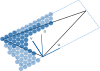
\includegraphics[width=0.4\textwidth]{images/triangle.pdf}
    \caption{Hexagonal sampling using pineda algorithm in local triangle space.}
    \label{fig:trianglesampling}
\end{figure}
We transform the sampled points back into global space by multiplying them by the transpose of the matrix in (\ref{eq:localtriangle}).

\subsection{Tension and Adhesion}
Surface tension effects are implemented according the method by Akinci et al. \cite{akinci2013}.
Akinci et al. define two types of forces, namely fluid cohesion and boundary adhesion. Fluid cohesion is an attractive force between particles. Macroscopically, it acts as a force field around the surface of the fluid which keeps the particles together. In this way surface tensions is realised and effects such as waterdroplets become arise. The adhesion force causes fluid particles to stick to solid boundaries, which results in a wetting effect.

\subsection{Surface Reconstruction}
To extract an explicit representation of the fluid surface, a signed distance function (SDF) \(\Phi(\mathbf{x}) \) describing the isosurface is required. We use the SPH method to approximate the isovalue at any arbitrary point \(\mathbf{x}\), depending on the normalized density \(\rho_j\) of the neighborhood particles \(j \in N\);
\begin{equation}
  \Phi(\mathbf{x})= \sum_{j \in N(\mathbf{x})}\frac{1}{\rho_j} W(||\mathbf{x} - \mathbf{x_j}|| / h) - c.
\end{equation}
The parameter \(c\) controls the zero level of the isosurface and therefore the enclosed volume of the explicit representation. We set \(c = 0.6\) during the remainder of the report. Using this method, we compute \(\Phi(\mathbf{x})\) at points in a grid and extract the triangle mesh representing the surface according to the Marching Cubes algorithm \cite{lorensen1987}.

% marching cubes


\subsection{Implementation}
The implementation uses a primarily imperative programming style with the exception of a few object oriented paradigms. Data encapsulation in the form of C++ classes is applied to ensure data consistency during computation. Basic inheritance is used to be able to reuse code for different parts of the program. This style of programming allows us to be flexible enough to incrementially implement the practical assignment tasks while sacrificing little to no performance due to design overload.
\begin{figure}[ht]
    \centering
    \includegraphics[width=0.5\textwidth]{images/system.pdf}
    \caption{Schematic overview of the implementation.}
    \label{fig:systemuml}
\end{figure}

The implementation is divided into two broad categories, systems and solvers. Figure \ref{fig:systemuml} gives a schematic UML diagram of the relation between the different parts of the implementation.
Systems include fluid particles and boundary particles, their generalization as particle systems and auxilary constructs. These implement the state and behaviour of fluid and boundary particles. A particlesystem is a collection of particles which are defined by their basic attributes, such as mass, density, position, velocity, etc. Particle systems are created via an Emitter object, which provides convience methods, such as creating particle systems from triangle meshes.
Every particle system is either a fluid system or a boundary system. Fluid and boundary systems hold additional attributes that are required to model behaviors that are unique to fluids and boundaries, respectively. As an example, boundary particles store information about the particle volumes and provide a method to compute the volume for each particle. All particle systems make use of precomputed lookup tables of the kernels. Since the kernel is evaluated multiple times per particle, the lookup tables are expected to provide significant speedups.

On the other hand, we have two seperate solvers for WCSPH and PBF. They aggregate fluid systems and boundary systems to model the progression of the given system. Both solvers share functions and general parameters over their superclass. Since the function that starts a simulation run is defined in the superclass, it is possible to determine the type of a solver at runtime.
In addition, each solver has been parallelized using OpenMP. To reduce the overhead from excessive creation and deletion of threads, a parallel region is created once upon entering an integration step. In this case, special care has to be taken to avoid race conditions due to shared memory between threads.

\section{Results}
\label{sec:results}
In this section, we run simple simulations to illustrate the differences between the WCSPH and the PBF solver. In Sec. \ref{subsec:comparison_general}, we provide a general comparison of the effects of fluid viscosity, boundary viscosity, surface tension and adhesion on both solvers by looking at dam break scenarios with different parameters. In Sec. \ref{subsec:comparison_tension} and Sec. \ref{subsec:comparison_adhesion} we take a closer look at minimal scenarios that showcase surface tension and 
adhesion. In Sec. \ref{subsec:comparison_smoothing}, Sec. \ref{subsec:sph_param_stiffness} and Sec. \ref{subsec:pbf_param_iterations} we return to dam break simulations to show the impact of XSPH smoothing and stiffness on the WCSPH solver and the impact of XSPH smoothing and the number of iterations on the PBF solver.  

%%%%%%%%%%%%%%%%%%%%%%%%%%%%%%%%%%%%%%%%%%%%%%%%%%%%%%%%%%%%%%%%%
%% General Dam Break
%%%%%%%%%%%%%%%%%%%%%%%%%%%%%%%%%%%%%%%%%%%%%%%%%%%%%%%%%%%%%%%%%
\subsection{Comparison: General}
\label{subsec:comparison_general}
In order to compare the characteristics of the WCSPH and the PBF solver and to showcase the impact of the parameters \texttt{fluid\_visc, boundary\_visc, tension} and \texttt{adhesion}, we simulated simple dam break scenarios with 74589 fluid particles using the WCSPH and the PBF solver. Fig. \ref{fig:dam_comparisons} shows frame 36 of these
simulations. In the simulations shown in panel 1 and panel 2, \texttt{tension} and \texttt{adhesion} were turned off and \texttt{fluid\_visc} and \texttt{boundary\_visc} were set to 0.001 to prevent their impact from covering up differences between the two solvers. When the fluid system is simulated using the WCSPH solver, it can be seen that
there are some fluid particles have higher velocities than their counterparts when the PBF solver was used. Consequently, fluid particles move up further along the y-axis - opposite to the direction of gravitational acceleration - when the WCSPH solver is used. The maximum particle densities during every frame of the simulations that are shown 
in panel 1 and panel 2 are plotted in Fig. \ref{fig:max_densities}. Over the first sixty frames of the simulations, the maximum particle density per frame is significantly higher when the WCSPH solver was used. The biggest deviation between the respective maximum densities was observed in frame 16, with maximum densities of approx. 
1100 $kg / m^3$ using the WCSPH solver and 1010 $kg / m^3$ using the PBF solver. 

In panels 3 and 4 of Fig. \ref{fig:dam_comparisons}, \texttt{fluid\_visc} was increased from 0.001 to 0.025. Increasing \texttt{fluid\_visc} hides the differences between the WCSPH and PBF solver that were observed in panels 1 and 2. Further, it can be seen that the height of the wave is smaller in panel 3 and 4 in comparison to panels 1 and 2
respectively, especially so for the simulations using the WCSPH solver (panel 1, panel 3).

In panels 5 and 6 of Fig. \ref{fig:dam_comparisons}, \texttt{fluid\_visc} was decreased back to 0.001 and \texttt{boundary\_visc} was increased to 0.025. As \texttt{fluid\_visc} is decreased, the differences between the WCSPH and PBF solver that were observed in panel 1 and panel 3 manifest themselves again. For both the WCSPH and PBF solver, 
there are more particles in proximity of the left boundary of the container when compared to panel 1 and panel 3. Additionally, the wave is narrower in panels 5 and 6. 

In panels 7 and 8 of Fig. \ref{fig:dam_comparisons}, \texttt{fluid\_visc} and \texttt{boundary\_visc} are set to 0.001 again and \texttt{tension} and \texttt{adhesion} are set to 0.25 and 10 respectively. Compared to panel 1 and panel 3 respectively, a fluid tongue forms as the wave crashes. As indicated by the darker color of the fluid particles, 
the densities of fluid particles at the top of the wave are higher for the WCSPH and PBF solver when \texttt{tension} and \texttt{adhesion} are turned on. Especially for the simulation using WCSPH, there are much less isolated fluid particles when \texttt{tension} is turned on. Comparing panels 5 and 6 with panels 7 and 8 respectively reveals the 
differences between boundary viscosity and adhesion: Particles in proximity of the boundary have lower density when boundary viscosity is used than when adhesion is used. To further illustrate the difference between \texttt{boundary\_visc} and \texttt{adhesion}, frame 160 of the same simulations that are shown in panels 5 to 8 are shown with a
different camera angle in panels 1 to 4 of Fig. \ref{fig:dam_comparisons_boundary_visc_adhesion}, respectively. It can be seen here that fluid particles that are in the proximity of the boundary sink back into the fluid again when using boundary viscosity with both the WCSPH and PBF solver. However, particles stay stuck to the container when adhesion
is used for both solvers. 

%%%%%%%%%%%%%%%%%%%%%%%%%%%%%%%%%%%%%%%%%%%%%%%%%%%%%%%%%%%%%%%%%
%% Tension
%%%%%%%%%%%%%%%%%%%%%%%%%%%%%%%%%%%%%%%%%%%%%%%%%%%%%%%%%%%%%%%%%
\subsection{Comparison: Tension}
\label{subsec:comparison_tension}

We simulated fluid cubes of 54872 particles in the absence of gravity to investigate the impact of surface tension on simulations using the WCSPH and PBF solver. Frame 53 of these simulations with \texttt{tension} set to 0, 0.25 and 1 is shown in Fig. \ref{fig:tension}. For both the WCSPH and the PBF solver, the fluid cube stays in its initial configuration
if \texttt{tension} is turned off. When \texttt{tension} is turned on, the fluid contracts into a spherical shape for both solvers. The higher the \texttt{tension} value, the faster this transition occurs. Generally, it seems like the spherical configuration is reached slightly faster when the PBF solver is used. It is important to note that when 
\texttt{tension} is turned on, the fluid reaches a spherical configuration in all of the simulations presented in Fig. \ref{fig:tension} eventually. An earlier frame was chosen in order to show how quickly the fluid cube contracts with different \texttt{tension} values. Lastly, the densities of the fluid particles are more uniform as the spherical configuration
is assumed when the PBF solver is used (see panels 2, 3, 5, 6).

%%%%%%%%%%%%%%%%%%%%%%%%%%%%%%%%%%%%%%%%%%%%%%%%%%%%%%%%%%%%%%%%%
%% Adhesion
%%%%%%%%%%%%%%%%%%%%%%%%%%%%%%%%%%%%%%%%%%%%%%%%%%%%%%%%%%%%%%%%%
\subsection{Comparison: Adhesion}
\label{subsec:comparison_adhesion}

In order to clearly demonstrate the effect of \texttt{adhesion} on the fluid simulation, we simulated a block of 67868 fluid particles falling onto an adhesive icosahedron using the WCSPH solver and the PBF solver. Fig. \ref{fig:adhesion} shows frame 160 of these simulations. For simulations using WCSPH, \texttt{adhesion} was set to 1, 2 and 5 in panels 1, 2 and 3 respectively. As the 
\texttt{adhesion} value is increased, the amount of fluid that is stuck to the icosahedron increases. In panel 3, the \texttt{adhesion} value is high enough to cause fluid particles that directly touch the icosahedron to almost resist gravity entirely. When \texttt{adhesion} is set to 2 (panel 2), access fluid drips down the icosahedron in a stream
that is narrower than the diameter of the icosahedron. This effect is still present when \texttt{adhesion} is set to 1 (panel 1), even though it is much less pronounced. For simulations using PBF, adhesion was set to 1, 3 and 10 in panels 4, 5 and 6, respectively. Again, more fluid particles are attached to the icosahedron as \texttt{adhesion} increases.
The streams of liquid that drip off the icosahedron are much smaller than the icosahedron diameter when \texttt{adhesion} is set to 3 and 10. However, the stream is narrower when the \texttt{adhesion} is set to 3 instead of 10. It is important to note that fluid still drops off when PBF is used with high  \texttt{adhesion} values. This was not the cases
for simulations using WCSPH. 

%%%%%%%%%%%%%%%%%%%%%%%%%%%%%%%%%%%%%%%%%%%%%%%%%%%%%%%%%%%%%%%%%
%% Smoothing
%%%%%%%%%%%%%%%%%%%%%%%%%%%%%%%%%%%%%%%%%%%%%%%%%%%%%%%%%%%%%%%%%
\subsection{Comparison: Smoothing}
\label{subsec:comparison_smoothing}
Multiple dam break scenarios 74589 were simulated using the WCSPH and PBF solver to investigate the impact of XSPH smoothing. Fig. \ref{fig:dam_comparisons_smoothing} shows frame 31 of these simulations. It is notable, that the differences that were observed between the WCSPH and the PBF solver in panels 1 and 2 of Fig. \ref{fig:dam_comparisons} are less pronounced when XSPH smoothing
is deactivated: Even in the simulation that used the PBF solver (panel 2), there are single particles with higher velocities than others. Increasing \texttt{xsph\_smoothing} to 1 leads to different outcomes depending on the used solver (panel 3, panel 4). Increasing XSPH smoothing only affects the behavior of the simulation to a small extent when the WCSPH solver is used. 
However, we observed fewer particles on the left side and more particles on the right side of the container when XSPH smoothing was activated. When the PBF solver is used, increasing XSPH smoothing causes the fluid particles to lose energy and have a more viscous appearance. There are barely any fluid particles that split off from the rest of the fluid body, when \texttt{xsph\_smoothing} is set to 1 and the PBF solver is used.   

%%%%%%%%%%%%%%%%%%%%%%%%%%%%%%%%%%%%%%%%%%%%%%%%%%%%%%%%%%%%%%%%%
%% Stiffness
%%%%%%%%%%%%%%%%%%%%%%%%%%%%%%%%%%%%%%%%%%%%%%%%%%%%%%%%%%%%%%%%%
\subsection{SPH Parameter: Stiffness}
\label{subsec:sph_param_stiffness}
When the WCSPH solver is used, the \texttt{stiffness} parameter can be tuned to impact the behavior of the simulation. Dam break simulations with 74589 fluid particles were run with \texttt{stiffness} set to 2500, 10000 and 25000. Frame 36 of the resulting simulations is shown in panels 1, 2 and 3 of Fig. \ref{fig:dam_comparisons_stiffness}, respectively. When \texttt{stiffness} is set to 2500 and 10000
the simulations are stable and look very similar to each other. However, increasing the stiffness to 25000 causes the simulation to become unstable.

%%%%%%%%%%%%%%%%%%%%%%%%%%%%%%%%%%%%%%%%%%%%%%%%%%%%%%%%%%%%%%%%%
%% Iterations
%%%%%%%%%%%%%%%%%%%%%%%%%%%%%%%%%%%%%%%%%%%%%%%%%%%%%%%%%%%%%%%%%
\subsection{PBF Parameter: Iterations}
\label{subsec:pbf_param_iterations}
When the PBF solver is used, the \texttt{nr\_iterations} that the PBF solver uses to minimize the density constraint can be set as a parameter. Dam break simulation with 74589 fluid particles were run with \texttt{nr\_iterations} set to 1, 3, 5, 7, 9 and 11. When \texttt{nr\_iterations} was set to 1 and 3, the simulations were stopped after five hours on frame 4 and 12, respectively. For both of these
simulations, the timestep that was dynamically calculated using the CFL condition became very small and prevented the simulation from progressing at a reasonble pace. When \texttt{nr\_iterations} was set to 5, 7, 9 and 11, the resulting simulations were very similar and hard to distinguish from each other. \texttt{max\_timestep} was set to 0.002s in all of the simulations in Fig. \ref{fig:dam_comparisons_iterations}. 
  
\begin{figure*}
  \centering
  \includegraphics[width=0.8\textwidth]{images/smallDam_IX_X.0036.png}
  \includegraphics[width=0.8\textwidth]{images/smallDam_XI_XII.0036.png}
  \caption{Frame 36 of simulations of 74589 fluid particles in a dam break scenario using the WCSPH and the PBF solver. In all simulations, a linear drag force of 0.02 was applied. For simulations using WCSPH, \texttt{max\_timestep = 0.0005s,
  xsph\_smoothing = 0.5, stiffness = 2500}. For simulations using PBF, \texttt{max\_timestep = 0.002s, xsph\_smoothing = 0.1, nr\_iterations = 7}. The other parameters were set as noted in the panels.}
  \label{fig:dam_comparisons}
\end{figure*}

\begin{figure*}
  \centering
  \includegraphics[width=\textwidth]{images/density_graphs.PNG}
  \caption{Max. density in $kg / m^3$ during every frame of the simulations in panel 1 and panel 2 of Fig. \ref{fig:dam_comparisons}.}
  \label{fig:max_densities}
\end{figure*}

\begin{figure*}
  \centering
  \includegraphics[width=\textwidth]{images/smallDam_XI_XII_tilted.0160.png}
  \caption{Frame 160 of simulations of 74589 fluid particles in a dam break scenario using the WCSPH and the PBF solver. In all simulations, a linear drag force of 0.02 was applied. For simulations using WCSPH, \texttt{max\_timestep = 0.0005s,
  xsph\_smoothing = 0.5, stiffness = 2500}. For simulations using PBF, \texttt{max\_timestep = 0.002s, xsph\_smoothing = 0.1, nr\_iterations = 7}. The other parameters were set as noted in the panels.}
  \label{fig:dam_comparisons_boundary_visc_adhesion}
\end{figure*}

\begin{figure*}
  \centering
  \includegraphics[width=\textwidth]{images/tension.0053.png}
  \caption{Frame 160 of simulations of 54872 particles arranged in a block without gravity using the WCSPH and the PBF solver. In all simulations, smoothing and gravity was disabled. For simulations using WCSPH, \texttt{max\_timestep = 0.0005s, stiffness = 2500, fluid\_visc = 0.001 }. 
  For simulations using PBF, \texttt{max\_timestep = 0.002s, nr\_iterations = 7, fluid\_visc = 0.001}. \texttt{tension} is set as indicated in the panels.}
  \label{fig:tension}
\end{figure*}

\begin{figure*}
  \centering
  \includegraphics[width=\textwidth]{images/iterations.0036.png}
  \caption{Frame 36 of simulations of 74589 fluid particles in a dam break scenario using the PBF solver. In all simulations, a linear drag force of 0.02 was applied and \texttt{max\_timestep = 0.002s, xsph\_smoothing = 0.1, fluid\_visc = 0.001, boundary\_visc = 0.001, tension = 0, adhesion = 0}. \texttt{nr\_iterations} was 
  set as noted in the panels. The simulations in panel 1 and panel 2 were interrupted after five hours of simulation on frame 4 and 12 respectively.}
  \label{fig:dam_comparisons_iterations}
\end{figure*}

\begin{figure*}
  \centering
  \includegraphics[width=\textwidth]{images/smoothing.0031.png}
  \caption{Frame 31 of simulations of 74589 fluid particles in a dam break scenario using the WCSPH and the PBF solver. In all simulations, a linear drag force of 0.02 was applied and \texttt{fluid\_visc = 0.001, boundary\_visc = 0.001, tension = 0, adhesion = 0}. For simulations using WCSPH, \texttt{max\_timestep = 0.0005s,
  stiffness = 2500}. For simulations using PBF, \texttt{max\_timestep = 0.002s, nr\_iterations = 7}. \texttt{xsph\_smoothing} was set as noted in the panels.}
  \label{fig:dam_comparisons_smoothing}
\end{figure*}

\begin{figure*}
  \centering
  \includegraphics[width=\textwidth]{images/stiffness.0036.png}
  \caption{Frame 36 of simulations of 74589 fluid particles in a dam break scenario using the WCSPH solver. In all simulations, a linear drag force of 0.02 was applied and \texttt{max\_timestep = 0.0005s, xsph\_smoothing = 0.5, fluid\_visc = 0.001, boundary\_visc = 0.001, tension = 0, adhesion = 0}. \texttt{stiffness} was 
  set as noted in the panels.}
  \label{fig:dam_comparisons_stiffness}
\end{figure*}

\begin{figure*}
  \centering
  \includegraphics[width=\textwidth]{images/adhesion.0160.png}
  \caption{Frame 160 of simulations of 67868 fluid particles falling onto an icosahedron using the WCSPH and the PBF solver with surface reconstruction. In all simulations, a linear drag force of 0.025 was applied. For simulations using WCSPH, \texttt{max\_timestep = 0.0005s,
  xsph\_smoothing = 0.25, stiffness = 2000, fluid\_visc = 0.01, boundary\_visc = 0.01, tension = 0.15}. For all simulations using the PBF solver \texttt{max\_timestep = 0.002s, xsph\_smoothing = 0.1, nr\_iterations = 7, fluid\_visc = 0.01, boundary\_visc = 0.005, tension = 0.1}. \texttt{adhesion} is set as noted in the panels.}
  \label{fig:adhesion}
\end{figure*}

\section{Discussion}
\label{sec:discussion}
In this section, we discuss the results that are documented in Sec. \ref{sec:results}. The general characteristics of the WCSPH and the PBF solver are discussed in Sec. \ref{disc:comparison_general}. The results of simulations using tension and adhesion are discussed in Sec. \label{disc:comparison_tension} and \label{disc:comparison_adhesion}.
The impact of XSPH smoothing, stiffness (WCSPH) and iterations (PBF) on the simulations are evaluated in Sec. \ref{disc:comparison_smoothing}, Sec. \ref{disc:comparison_stiffness} and Sec. \ref{disc:comparison_iterations}, respectively.

\subsection{Comparison: General}
\label{disc:comparison_general}
A solution to the Navier-Stokes equation can be numerically approximated using WCSPH (Sec. \ref{subsec:wcsph}) and PBF (Sec. \ref{subsec:pbf}). In order to showcase the differences between these two solvers, their general characteristics were investigated in Sec. \ref{subsec:comparison_general}. As described in Sec. \ref{subsec:comparison_general},
it is more common to find single particles with a lot of energy when WCSPH is used. Hand in hand, we observed that the maximum particle density tends to be higher when the WCSPH solver is used (Fig. \ref{fig:max_densities}). As big positive deviations of the a particle's density from rest density cause big pressure terms in WCSPH (Eq. \ref{eq:pressure}), we suggest that
the increased particle velocity in WCSPH results from violations of the fluid incompressibility during the simulation. This is in accordance with \cite{macklin2013}, where the maximum fluid density is used as a measure for fluid compressibility. On the other hand, PBF approximates a solution to the density constraint (Eq. \ref{eg:pbfconstraint}) during 
every simulation step. This explains why the maximum densities in Fig. \ref{fig:max_densities} are smaller when the PBF solver is used. As a result, fluid incompressibility is not violated as much as when the WCSPH solver is used. Consequently, single particles with increased energy are rare with the PBF solver.  

Increasing the fluid viscosity reduces the energy in the system and increases the stability of the simulation (Fig. \ref{fig:dam_comparisons}, panels 3, 4). This was to be expected, as fluid viscosity is added to model internal friction of the fluid. Especially for WCSPH, the results of the simulation change notably when fluid viscosity is increased. Due 
to the interal friction, fluid particles move slower, consequently making it harder for fluid particles to get too close to each other during one simulation step. Thus, it is less likely that the fluid incompressibility is violated when fluid viscosity is used in the simulation, which would blow up pressure terms unreasonably (see. Eq. \ref{eq:pressure}).

While investigating the difference between the effects of boundary viscosity and adhesion (Fig. \ref{fig:dam_comparisons}, panels 5, 6, 7, 8), we noticed that fluid particles that are close to the boundary have higher densities when adhesion is used in comparison to boundary viscosity. One likely explanation for this phenomenon is that adhesion models an attractive
force between boundary and fluid particles \cite{akinci2013}, whereas boundary viscosity merely models friction between boundary and fluid particles \cite{akinci2012}. Thus, the distance between boundary and fluid particles when adhesion is used is smaller than their distance when boundary viscosity is used, leading to a higher particle density. This would be in line with the 
observations from Fig. \ref{fig:dam_comparisons_boundary_visc_adhesion}, where fluid particles stick to boundary particles when adhesion is used, but not when boundary viscosity is used.

%%%%%%%%%%%%%%%%%%%%%%%%%%%%%%%%%%%%%%%%%%%%%%%%%%%%%%%%%%%%%%%%%
%% Tension
%%%%%%%%%%%%%%%%%%%%%%%%%%%%%%%%%%%%%%%%%%%%%%%%%%%%%%%%%%%%%%%%%
\subsection{Comparison: Tension}
\label{disc:comparison_tension}
Surface tension is caused by cohesive forces among neighboring fluid particles \cite{akinci2013}. Fluid particles on the surface of the fluid do not have neighbors on all sides and are thus pulled inwards. This matches the observations that were made while simulating a fluid cube with surface tension in the absence of gravity (Fig. \ref{fig:tension}).
As expected, fluid particles were not pulled inwards when surface tension was turned off, causing the cube to stay in its initial configuration. The higher the \texttt{tension} value, the faster the cube assumed a spherical configuration. The fact that the spherical configuration was assumed slower and that the particle densities were less uniform
when using the WCSPH solver could have the same underlying cause: As discussed in Sec. \ref{disc:comparison_general}, the WCSPH is prone to violating fluid incompressibility. As surface tension draws particles closer to each other, their densities become too high and they might push particles slightly outwards again. However, this hypothesis would 
have to be tested more thoroughly, possibly by taking a closer look at particle densities throughout the simulations using WCSPH. 

%%%%%%%%%%%%%%%%%%%%%%%%%%%%%%%%%%%%%%%%%%%%%%%%%%%%%%%%%%%%%%%%%
%% Adhesion
%%%%%%%%%%%%%%%%%%%%%%%%%%%%%%%%%%%%%%%%%%%%%%%%%%%%%%%%%%%%%%%%%
\subsection{Comparison: Adhesion}
\label{disc:comparison_adhesion}
As briefly discussed in Sec. \ref{disc:comparison_general}, adhesion models an attractive force between boundary and fluid particles \cite{akinci2013}. In Fig. \ref{fig:adhesion} we observed that the higher the \texttt{adhesion} value, the more fluid is attached to the icosahedron for both WCSPH and PBF, which matches our expectations. 
Interestingly, when \texttt{adhesion} is set to 5 with the WCSPH solver, the fluid particles that touched the icosahedron became almost entirely stuck to it, even resisting gravitational forces. This suggests that adhesion forces are stronger when the WCSPH solver is used in comparison to the PBF solver. It is important to note that the opposite observation
was made in Sec. \ref{disc:comparison_tension} while discussing surface tension. One possible hypothesis could be that fluid particles are dragged down the icosahedron by neighboring fluid particles due to stronger tension forces, which overcome even higher adhesion values when the PBF solver is used. 

Further, it is remarkable that the diameter of the fluid stream that drips down the icosahedron does not decrease as \texttt{adhesion} is increased from 5 to 10 with the PBF solver. One possible explanation could be that an \texttt{adhesion} of 10 causes one layer of fluid particles to be stuck to the surface of the icosahedron entirely. The fluid particles
in the stream that drips down the icosahedron would thus be blocked off from the boundary, leading to a smaller adhesive force. However, this would raise the question why there are areas on the surface of the icosahedron that were clearly touched by fluid before, but do not have any attached to it in the current frame. Such areas could be found e.g. at the top
of the icosahedron. Finally, if this hypothesis were true, we would expect a similar behavior for the simulation using WCSPH and an \texttt{adhesion} of 5.

%%%%%%%%%%%%%%%%%%%%%%%%%%%%%%%%%%%%%%%%%%%%%%%%%%%%%%%%%%%%%%%%%
%% Smoothing
%%%%%%%%%%%%%%%%%%%%%%%%%%%%%%%%%%%%%%%%%%%%%%%%%%%%%%%%%%%%%%%%%
\subsection{Comparison: Smoothing}
\label{disc:comparison_smoothing}
According to \cite{monaghan1989}, XSPH smoothing can be used to ensure that particles that are close to each other will have nearly identical velocities. This helps preventing regions where SPH particles pass through each other without increasing fluid viscosity. In our experiments in Fig. \ref{fig:dam_comparisons_smoothing}, we observed that particles velocities 
indeed seem to be closer to their neighbors' velocities when XSPH smoothing is used. However, this effect was much more pronounced for the PBF solver. Most likely, this can be attributed to the fact that smoothing is applied without taking pressure forces into account in PBF. Consequently, most particle velocities that are used for XSPH smoothing in the PBF solver have smaller
magnitudes than their counterparts in the WCSPH solver. As a result, the absolute difference between velocities of neighboring particles after XSPH smoothing is much smaller for the PBF solver. If the density constraint was already minimized in the previous timestep, the $\Delta x$ that are calculated during the constraint minimization of the current timestep will be small.
Overall, this leads to a loss in energy when PBF and XSPH smoothing are used together. In \cite{schechter2012}, XSPH smoothing is used to artificially introduce viscosity in fluid simulations using an SPH solver. We were not able to observe more viscous fluid behavior when XSPH smoothing was used with the WCSPH solver. Maybe it is worth investigating the effects of smoothing
on the WCSPH solver in simulations with a smaller stiffness value again.

%%%%%%%%%%%%%%%%%%%%%%%%%%%%%%%%%%%%%%%%%%%%%%%%%%%%%%%%%%%%%%%%%
%% Stiffness
%%%%%%%%%%%%%%%%%%%%%%%%%%%%%%%%%%%%%%%%%%%%%%%%%%%%%%%%%%%%%%%%%
\subsection{SPH Parameter: Stiffness}
\label{disc:comparison_stiffness}
In the WCSPH solver, the particle pressures are computed by multiplying positive deviations in particle density from rest density with a \texttt{stiffness} constant (Eq. \ref{eq:pressure}). Thus, the higher the \texttt{stiffness} constant, the higher the resulting particle pressures, which in turn leads
to higher particle velocities. In Sec. \ref{subsec:sph_param_stiffness} we observed that the difference between simulations with \texttt{stiffness} set to 2500 and 10000 were minor. However, if the \texttt{stiffness} is set to 25000 the simulation becomes instable. \cite{solenthaler09} suggest that 
higher \texttt{stiffness} values require lower timesteps. It is possible that the simulation with \texttt{stiffness} set to 25000 would be stable, if the timestep was decreased accordingly. On the other hand, if the timestep was increased, it is plausible that the simulation with \texttt{stiffness} set 
to 10000 would become instable as well.


%%%%%%%%%%%%%%%%%%%%%%%%%%%%%%%%%%%%%%%%%%%%%%%%%%%%%%%%%%%%%%%%%
%% Iterations
%%%%%%%%%%%%%%%%%%%%%%%%%%%%%%%%%%%%%%%%%%%%%%%%%%%%%%%%%%%%%%%%%
\subsection{PBF Parameter: Iterations}
\label{disc:comparison_iterations}
During every simulation step with the PBF solver, the density constraints (Eq. \ref{eg:pbfconstraint}) are minimized iteratively \cite{macklin2013}. Increasing the number of iterations trades runtime performance of the simulation for lower compressibility of the fluid. In Sec. \ref{subsec:pbf_param_iterations}, we observed
that simulations are almost identical regardless of the exact number of iterations, as long as the number of iterations is sufficiently high. In Fig. \ref{fig:dam_comparisons_iterations}, this was the case for all simulations that used at least five iterations per simulation step. Simulations that used
an insufficient number of iterations stopped progressing at a reasonable pace after few frames, as the timestep that was dynamically calculated using the CFL condition approached 0s. This is due to excessive particle velocities. Particle velocities are expected to explode if an insufficient number of iterations
is used in the PBF solver, as a particle that has high density after a position update without pressure forces will have a significant position changes in the first couple of iterations. As the particle velocity directly depends on these position changes, the new particle velocity will be big as well.  

\section{Conclusion}
\label{sec:conclusion}

% respong to introduction and discuss implications of result


\section{Outlook}
\label{sec:future}
The WCSPH and PBF implementation as well as the surface reconstruction offers a high level of concurency in the form of data parallelism. This means, that there are many parts in the programm where sequentially processed data can be split into independant groups which can be processed in parallel.

% what are the next steps?
% what did we learn from this and how could we apply this for the future?



\bibliographystyle{alpha}
{\footnotesize
\bibliography{references.bib}}


% tables, if needed, are like this.
% \begin{table}[ht]
% \begin{tabular}{|l|l|l|}
% \hline
% Time (s) & Distance (m) & Charge (C) \\ \hline
% 0        & 0            & 10         \\ \hline
% 1        & 1            & 5          \\ \hline
% 2        & 4            & 6          \\ \hline
% \end{tabular}
% \caption{An example table.}
% \label{table:ExampleTable}
% \end{table}

% \begin{figure}[ht]
%     \centering
%     \includegraphics[width=0.5\textwidth]{img/generic_plot.pdf}
%     \caption{Here is a caption for a figure.}
%     \label{fig:ExampleFigure}
% \end{figure}

\end{document}

%%% Local Variables:
%%% mode: latex
%%% TeX-master: t
%%% End:
